
\begin{figure}[ht]
    \centering
    \subfloat[Ablation studies on the number of transformer encoder block layers.]{
        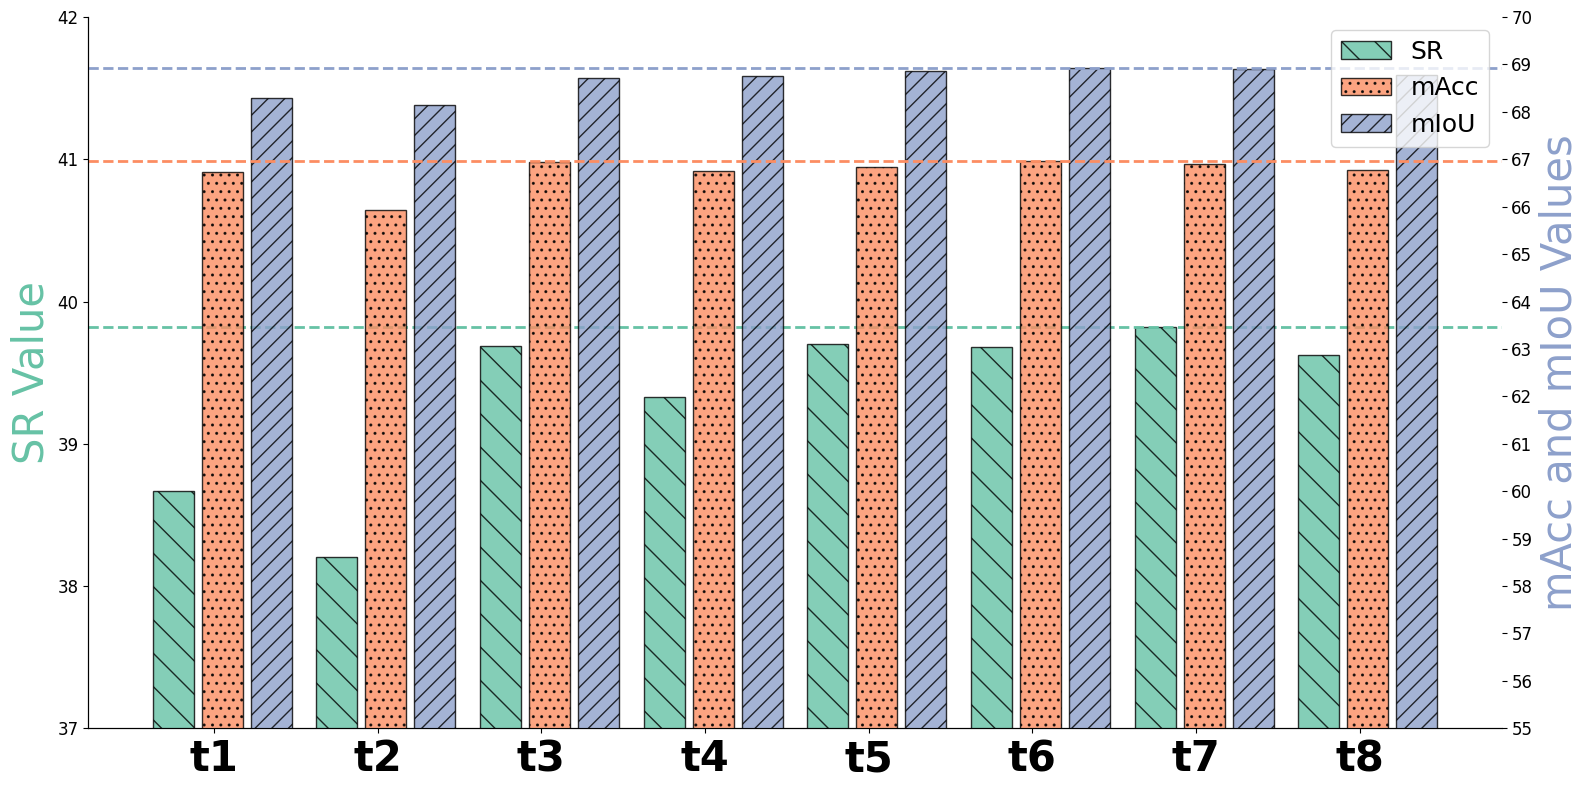
\includegraphics[width=0.48\textwidth, keepaspectratio]{figures/ab1.png}
        \label{fig:num_trans}
    }
    \hfill
    \subfloat[Ablation studies on the scale of mask loss.]{
        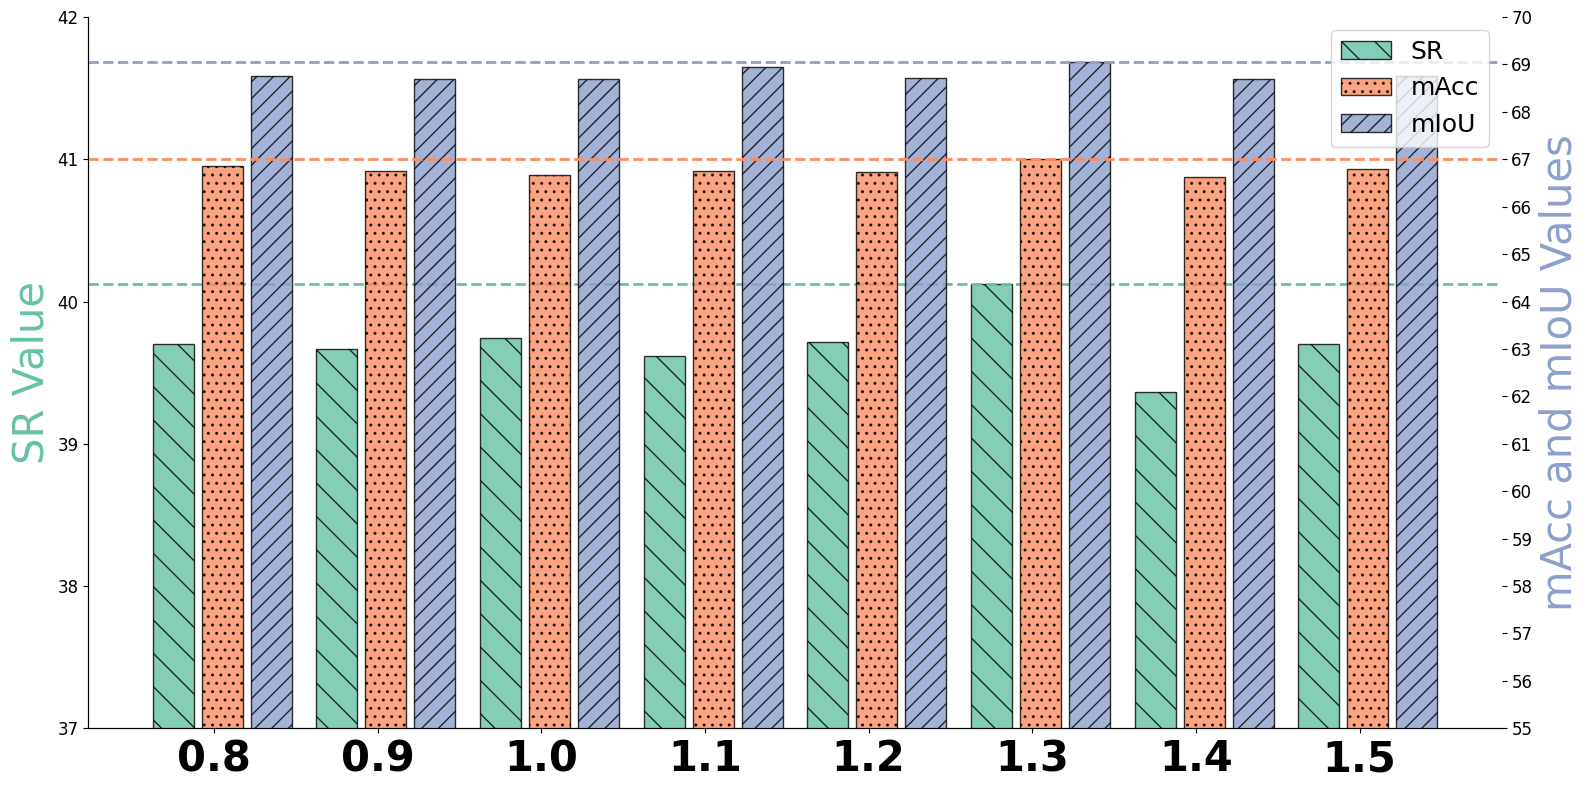
\includegraphics[width=0.48\textwidth, keepaspectratio]{figures/ab2.png}
        \label{fig:scale_mask}
    }
    \hfill
    \subfloat[Ablation studies on the weights coefficient of loss.]{
        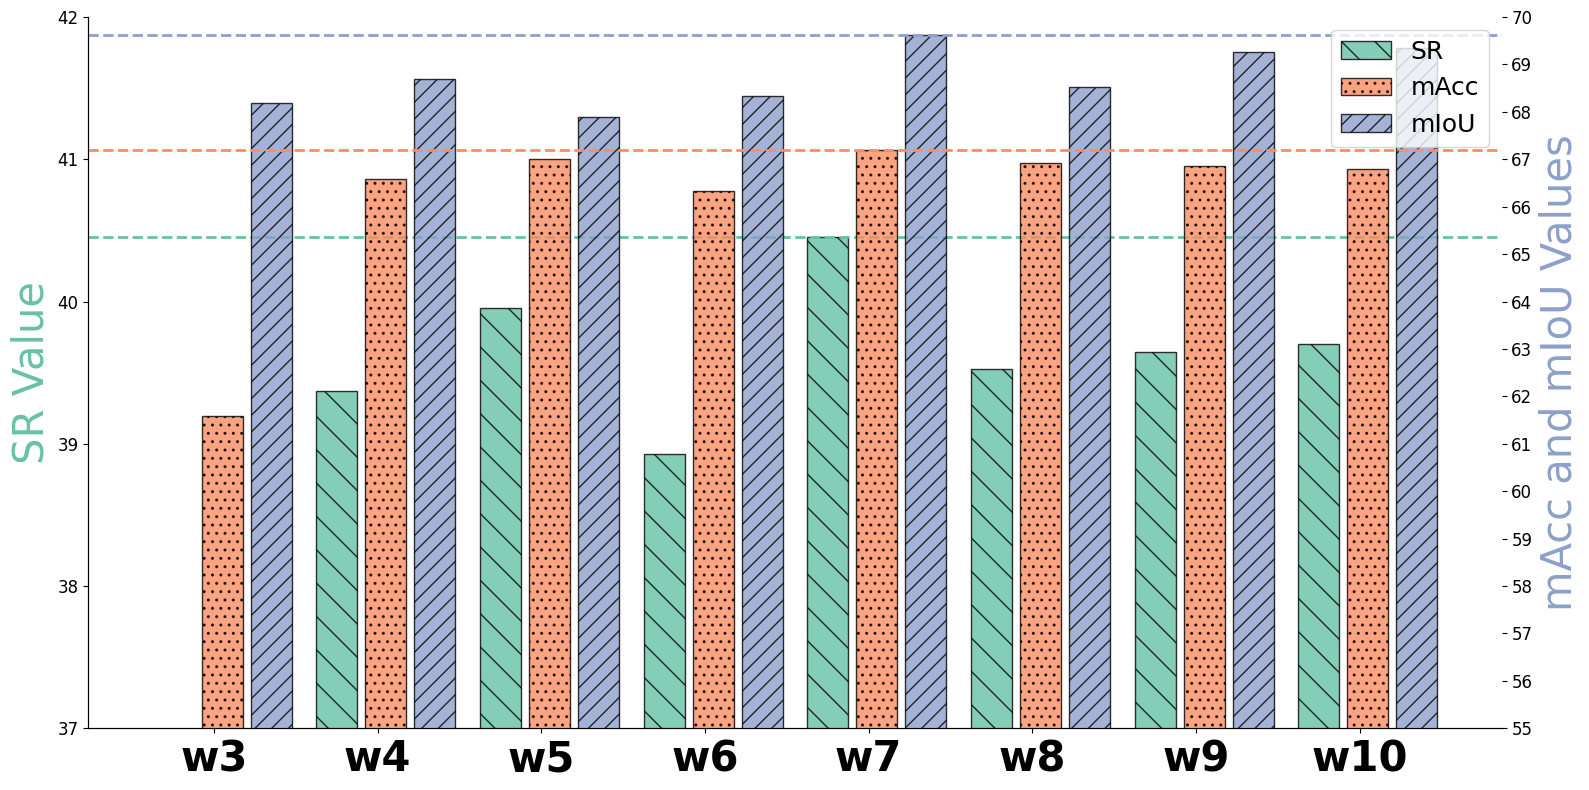
\includegraphics[width=0.48\textwidth, keepaspectratio]{figures/ab3.png}
        \label{fig:wei_coef}
    }
    \caption{Combined ablation studies of different coefficients. Note: ``t1'' refers to the number of transformer encoder layers in \Cref{fig:num_trans}; ``0.8'' represents the value of $\rho$ in loss function in \Cref{fig:scale_mask}; and ``w3'' indicates the value of the gradient-weighted loss $w_0$ in \Cref{fig:wei_coef}.   }
    \label{fig:combined}
\end{figure}